\documentclass{urdpl}     % praca w języku polskim

% Lista wszystkich języków stanowiących języki pozycji bibliograficznych użytych w pracy.
% (Zgodnie z zasadami tworzenia bibliografii każda pozycja powinna zostać utworzona zgodnie z zasadami języka, w którym dana publikacja została napisana.)
\usepackage[english,polish]{babel}

% Użyj polskiego łamania wyrazów (zamiast domyślnego angielskiego).
\usepackage{polski}

\usepackage[utf8]{inputenc}

% dodatkowe pakiety

\usepackage{mathtools}
\usepackage{amsfonts}
\usepackage{amsmath}
\usepackage{amsthm}
\usepackage[hidelinks]{hyperref}
\usepackage{float}
\usepackage{listings}
\usepackage{graphicx}
\usepackage{subcaption}
\usepackage{booktabs} % Dla \toprule, \midrule, \bottomrule
\usepackage{multirow} 
\usepackage{tabularx} 
\usepackage{amssymb} 
\usepackage{listings}
\usepackage{xcolor}
\usepackage{array}
\usepackage{makecell}
\usepackage[flushleft]{threeparttable}
\usepackage[normalem]{ulem}
\usepackage{lineno}
\usepackage{pdfpages}
% ---------------------------------------------

% --- < bibliografia > ---

\usepackage{csquotes}

% ------------------------
% --- < listingi > ---

% Użyj czcionki kroju Courier.
\usepackage{courier}

\usepackage{listings}
\lstloadlanguages{TeX}
\renewcommand{\lstlistlistingname}{Spis listingów}
\renewcommand{\lstlistingname}{Listing}


\lstset{
	literate={ą}{{\k{a}}}1
           {ć}{{\'c}}1
           {ę}{{\k{e}}}1
           {ó}{{\'o}}1
           {ń}{{\'n}}1
           {ł}{{\l{}}}1
           {ś}{{\'s}}1
           {ź}{{\'z}}1
           {ż}{{\.z}}1
           {Ą}{{\k{A}}}1
           {Ć}{{\'C}}1
           {Ę}{{\k{E}}}1
           {Ó}{{\'O}}1
           {Ń}{{\'N}}1
           {Ł}{{\L{}}}1
           {Ś}{{\'S}}1
           {Ź}{{\'Z}}1
           {Ż}{{\.Z}}1,
	basicstyle=\footnotesize\ttfamily,
}

% defninicja stylu python
\lstdefinestyle{stylePython}{
    language=Python,
    commentstyle=\color{green},          % Kolor komentarzy
    keywordstyle=\color{blue},           % Kolor słów kluczowych
    numberstyle=\tiny\color{gray},       % Kolor i styl numerów linii
    stringstyle=\color{red},             % Kolor ciągów znaków
    basicstyle=\ttfamily\footnotesize,   % Podstawowy styl kodu
    breakatwhitespace=false,             % Automatyczne dzielenie wierszy
    breaklines=true,                     % Dzielenie długich linii
    keepspaces=true,                     % Zachowanie spacji
    numbers=left,                        % Numery linii po lewej
    numbersep=5pt,                       % Odstęp numerów od kodu
    showspaces=false,                    % Nie pokazuj spacji
    showstringspaces=false,              % Nie pokazuj spacji w ciągach znaków
    showtabs=false,                      % Nie pokazuj tabulacji
    tabsize=2                            % Rozmiar tabulacji
}

% defnicja stylu JAVA
\lstdefinestyle{javaStyle}{
    language=Java,
    basicstyle=\ttfamily\footnotesize,
    keywordstyle=\color{blue},
    commentstyle=\color{green!50!black}\itshape,
    stringstyle=\color{green},
    numberstyle=\tiny\color{gray},
    numbers=left,
    numbersep=5pt,                       % Odstęp numerów od kodu
    stepnumber=1,
    showspaces=false,                    % Nie pokazuj spacji
    tabsize=2,
    showstringspaces=false,
    breaklines=true,
    breakatwhitespace=false,             % Automatyczne dzielenie wierszy
    showtabs=false,                      % Nie pokazuj tabulacji
    keepspaces=true                    % Zachowanie spacji
}


\definecolor{stringcolor}{RGB}{163,21,21}    % pomarańczowy - stringi
\definecolor{typecolor}{RGB}{43, 145, 176}     % ciemny fiolet - klasy, typy

\lstdefinestyle{csStyle}{
    language=[Sharp]C, % dla C#; można zmienić na Java
    basicstyle=\ttfamily\footnotesize,
    keywordstyle=\color{blue},
    stringstyle=\color{stringcolor},
    commentstyle=\color{green!50!black}\itshape,
    morekeywords={class, public, private, protected, static, void, string, int, new}, % dodatkowe słowa kluczowe
    emphstyle=\color{typecolor}\bfseries, % klasy na fioletowo
    numbers=left,
    numbersep=5pt,                       % Odstęp numerów od kodu
    numberstyle=\tiny\color{gray},
    stepnumber=1,
    breaklines=true,
    showspaces=false,                    % Nie pokazuj spacji
    tabsize=2,
    showstringspaces=false,
    breakatwhitespace=false,             % Automatyczne dzielenie wierszy
    showtabs=false,                      % Nie pokazuj tabulacji
    keepspaces=true                    % Zachowanie spacji  
}

\definecolor{lightgray}{rgb}{0.9,0.9,0.9}
    % \definecolor{blue}{rgb}{0,0,1}
    \definecolor{green}{rgb}{0,0.6,0}
    % \definecolor{red}{rgb}{0.6,0,0}
    \definecolor{gray}{rgb}{0.5,0.5,0.5}

% % ------------------------
\AtBeginDocument{
	\renewcommand{\tablename}{Tabela}
	\renewcommand{\figurename}{Rys.}   
    \newcommand{\listingname}{Listing}
}


% ------------------------
% --- < tabele > ---

% defines the X column to use m (\parbox[c]) instead of p (`parbox[t]`)
\newcolumntype{C}[1]{>{\hsize=#1\hsize\centering\arraybackslash}X}

%---------------------------------------------------------------------------
\begin{document}


\begin{titlepage}
    \begin{flushleft}
        \textbf{UNIWERSYTET RZESZOWSKI}\\
        \textbf{WYDZIAŁ NAUK ŚCISŁYCH I TECHNICZNYCH}\\
        \textbf{INSTYTUT INFORMATYKI}
    \end{flushleft}
    
    % Logo po prawej
    \begin{flushright}
        
\includegraphics[width=3cm]{logour.png}
    \end{flushright}

    \vspace{5cm}

    \begin{center}
        \textit{Jakub Pelic}\\
        \textit{134957}\\
        \textit{Informatyka}
    \end{center}
\vspace{2\baselineskip}
        \begin{center}
        \textbf{Dokumentacja Aplikacji Do Zarządzania Drużyną Piłkarską}\\
    \end{center}
    \vspace{2\baselineskip}

\begin{center}
    Praca projektowa \\
    Praca wykonana pod kierunkiem \\
    mgr inż. Ewa Żesławska
\end{center}

    \vfill

    \begin{center}
        \textit{Rzeszów 2025r.}
    \end{center}

\end{titlepage}

\tableofcontents

\chapter{Opis założeń projektu}

Celem projektu jest stworzenie aplikacji desktopowej umożliwiającej użytkownikowi zarządzanie drużynami piłkarskimi i ich zawodnikami. Aplikacja została napisana w języku Java z wykorzystaniem biblioteki Swing do tworzenia interfejsu graficznego oraz JDBC do komunikacji z bazą danych MySQL. Program umożliwia tworzenie kont użytkowników, logowanie się, tworzenie i edycję drużyn oraz zarządzanie listą zawodników. Głównym problemem, który rozwiązuje aplikacja, jest brak prostych i intuicyjnych narzędzi desktopowych dla amatorskich trenerów lub pasjonatów piłki nożnej, którzy chcą w prosty sposób śledzić skład i strukturę drużyn. Potrzeba ta została zaobserwowana na poziomie amatorskich lig, szkółek piłkarskich oraz entuzjastów lokalnych rozgrywek, którzy dotychczas korzystają z arkuszy kalkulacyjnych lub ręcznych zapisków, co nie jest efektywne ani wygodne.

W celu rozwiązania tego problemu, projekt zakłada stworzenie kompletnego systemu desktopowego, który po zalogowaniu się użytkownika umożliwia zarządzanie jego drużynami. Każdy użytkownik może dodawać, edytować i usuwać drużyny, a także modyfikować ich skład osobowy poprzez dodawanie lub usuwanie zawodników. Proces rozpoczyna się od formularza logowania, skąd można przejść do rejestracji nowego konta. Po pomyślnym zalogowaniu użytkownik widzi listę swoich drużyn. Funkcje dodawania i edycji otwierają osobne okna formularzy. Całość została zaprojektowana w sposób obiektowy — każda klasa GUI dziedziczy po klasie nadrzędnej odpowiedzialnej za wspólne ustawienia graficzne (takie jak centrowanie okna). Logika interakcji została rozdzielona pomiędzy kontrolery przypisane do każdego widoku.

Aplikacja wymaga aktywnego połączenia z bazą danych MySQL, co oznacza, że użytkownik musi posiadać zainstalowany serwer bazy danych oraz odpowiednio skonfigurowany dostęp (login i hasło). Rezultatem prac projektowych jest w pełni funkcjonalna aplikacja komputerowa, którą można rozszerzać o nowe funkcjonalności w przyszłości (np. statystyki zawodników, harmonogramy meczów).

\section{Wymagania funkcjonalne}

\begin{itemize}
  \item Możliwość rejestracji nowego użytkownika z podaniem wszystkich niezbędnych danych.
  \item Możliwość logowania do aplikacji po uprzednim utworzeniu konta.
  \item Przechowywanie i weryfikacja danych logowania w bazie danych MySQL.
  \item Lista drużyn przypisana do zalogowanego użytkownika.
  \item Możliwość dodania nowej drużyny poprzez wypełnienie formularza.
  \item Możliwość edycji nazwy wybranej drużyny.
  \item Możliwość usunięcia wybranej drużyny.
  \item Wyświetlanie listy zawodników przypisanych do konkretnej drużyny.
  \item Możliwość dodania zawodnika do wybranej drużyny (z podaniem imienia i nazwiska).
  \item Możliwość usunięcia zawodnika z drużyny.
  \item Oddzielenie warstwy GUI od logiki poprzez zastosowanie kontrolerów.
\end{itemize}

\section{Wymagania niefunkcjonalne}

\begin{itemize}
  \item Aplikacja powinna być dostępna na systemie operacyjnym Windows z zainstalowanym środowiskiem Java.
  \item Interfejs użytkownika powinien być intuicyjny i spójny wizualnie (wspólna klasa Frame dla okien).
  \item Wszystkie działania powinny być możliwe do wykonania w czasie krótszym niż 3 sekundy.
  \item System musi być odporny na błędy związane z brakiem połączenia z bazą danych.
  \item Aplikacja powinna przechowywać dane w lokalnej bazie danych MySQL.
  \item Zmiany wprowadzane w interfejsie powinny być natychmiastowo odzwierciedlane w bazie danych.
  \item Aplikacja powinna umożliwiać łatwe aktualizacje i konserwację kodu dzięki modularnej strukturze klas.
  \item W przypadku błędnych danych logowania aplikacja powinna poinformować użytkownika o niepowodzeniu.
  \item Okna aplikacji powinny być automatycznie centrowane na ekranie użytkownika.
\end{itemize}

\chapter{Opis struktury projektu}

Struktura projektu została zaprojektowana w sposób modularny z wyraźnym podziałem na warstwę logiki (kontrolery), interfejs użytkownika (GUI) oraz logikę biznesową (modele danych). Aplikacja została zrealizowana w języku Java z wykorzystaniem środowiska IntelliJ IDEA oraz bibliotek Swing (do tworzenia interfejsu graficznego) i JDBC (do obsługi połączenia z bazą danych MySQL).

\section{Struktura klas}

Projekt składa się z następujących typów plików:

\begin{itemize}
  \item \textbf{GUI (.java + .form)} – klasy odpowiedzialne za interfejs graficzny: \texttt{AplikacjaGUI}, \texttt{DodajPilkarzaGUI}, \texttt{DodawanieDruzynyGUI}, \texttt{EdytyujDruzyneGUI}, \texttt{LoginGUI}, \texttt{RejestracjaGUI}, każda posiada odpowiadający plik \texttt{.form} (projekt wizualny).
  \item \textbf{Kontrolery} – klasy zarządzające logiką aplikacji: \texttt{AplikacjaController}, \texttt{DodajPilkarzaController}, \texttt{DodawanieDruzynyController}, \texttt{EdytyujDruzyneController}, \texttt{LoginController}, \texttt{RejestracjaController}.
  \item \textbf{Modele danych} – klasy reprezentujące dane aplikacji: \texttt{Druzyna}, \texttt{Pilkarz}, \texttt{Uzytkownik}.
  \item \textbf{Pozostałe klasy wspomagające} – \texttt{Main} (punkt wejścia aplikacji), \texttt{Frame} (bazowa klasa okien aplikacji), \texttt{Komunikat} (wyświetlanie informacji użytkownikowi), \texttt{BazaDanych} (zarządzanie połączeniem z MySQL).
\end{itemize}

\section{Hierarchia klas i logika aplikacji}

\begin{itemize}
  \item Wszystkie klasy graficzne dziedziczą po klasie \texttt{Frame}, która ustawia wspólne parametry okien, takie jak centrowanie na ekranie.
  \item Klasa \texttt{Main} uruchamia aplikację i wywołuje ekran logowania.
  \item Klasa \texttt{LoginGUI} umożliwia logowanie użytkownika, a \texttt{LoginController} obsługuje logikę uwierzytelniania (porównanie danych z bazą).
  \item Klasa \texttt{RejestracjaGUI} umożliwia rejestrację nowego użytkownika, a \texttt{RejestracjaController} zapisuje dane do bazy.
  \item Po zalogowaniu uruchamiane jest główne okno \texttt{AplikacjaGUI}, zarządzane przez \texttt{AplikacjaController}, wyświetlające drużyny i umożliwiające ich modyfikację.
  \item Dodawanie/edycja drużyn realizowana jest w osobnych oknach: \texttt{DodawanieDruzynyGUI}, \texttt{EdytujDruzyneGUI}.
  \item Analogicznie, zawodników obsługują: \texttt{DodajPilkarzaGUI}, \texttt{DodajPilkarzaController}.

\end{itemize}

\subsection{Opis metod kontrolerów}

\textbf{AplikacjaController}
\begin{itemize}
  \item \texttt{OdswiezListeDruzyn()} – Pobiera z bazy danych listę drużyn przypisanych do zalogowanego użytkownika i wyświetla je w interfejsie.
  \item \texttt{DodajDruzyneObsluga()} – Otwiera nowe okno do dodania drużyny i zamyka bieżące.
  \item \texttt{UsunDruzyne()} – Usuwa zaznaczoną drużynę z bazy danych i z listy GUI.
  \item \texttt{EdytujDruzyne()} – Przechodzi do okna edycji wybranej drużyny.
\end{itemize}

\textbf{RejestracjaController}
\begin{itemize}
  \item \texttt{Zarejestuj()} – Obsługuje proces rejestracji nowego użytkownika: sprawdza poprawność danych i zapisuje je do bazy.
  \item \texttt{CzyIstniejeTakiUzytkownik(String login)} – Sprawdza, czy użytkownik o podanym loginie już istnieje w bazie.
  \item \texttt{Wroc()} – Powrót do okna logowania.
\end{itemize}

\textbf{LoginController}
\begin{itemize}
  \item \texttt{Zaloguj()} – Autoryzuje dane logowania użytkownika na podstawie zapytania SQL. W przypadku powodzenia przechodzi do głównego okna aplikacji.
\end{itemize}

\textbf{DodawanieDruzynyController}
\begin{itemize}
  \item \texttt{DodajDruzyne()} – Dodaje nową drużynę do bazy, jeśli taka jeszcze nie istnieje.
  \item \texttt{CzyIstniejeTakaDruzyna(String nazwa)} – Sprawdza, czy drużyna o danej nazwie znajduje się już w bazie danych.
  \item \texttt{Wroc()} – Powrót do głównego okna aplikacji.
\end{itemize}

\textbf{EdytujDruzyneController}
\begin{itemize}
  \item \texttt{ZmienNazwe()} – Zmienia nazwę wybranej drużyny w bazie danych.
  \item \texttt{DodajPilkarza()} – Otwiera okno dodawania nowego piłkarza do danej drużyny.
  \item \texttt{UsunPilkarza()} – Usuwa zaznaczonego piłkarza z bazy i z listy GUI.
  \item \texttt{Wroc()} – Powrót do głównego okna aplikacji.
  \item \texttt{OdswiezListePilkarzy()} – Wczytuje wszystkich piłkarzy przypisanych do danej drużyny i wyświetla ich w interfejsie.
\end{itemize}

\textbf{DodajPilkarzaController}
\begin{itemize}
  \item \texttt{Dodaj()} – Dodaje nowego piłkarza do bazy danych i przypisuje go do konkretnej drużyny.
  \item \texttt{Wroc()} – Powrót do głównego okna aplikacji.
\end{itemize}


\subsection{Wykorzystane technologie}

\begin{itemize}
  \item \textbf{Java 24} – język programowania.
  \item \textbf{Swing} – biblioteka do budowy GUI.
  \item \textbf{JDBC} – interfejs do obsługi bazy danych.
  \item \textbf{MySQL 10.4.32-MariaDB} – relacyjna baza danych przechowująca dane użytkowników, drużyn i zawodników.
  \item \textbf{IntelliJ IDEA 2025.1} – środowisko programistyczne wykorzystywane do budowy projektu.
\end{itemize}

\subsection{Zarządzanie danymi i baza danych}

Dane przechowywane są w lokalnej bazie danych MySQL. Struktura bazy obejmuje  trzy tabele:
\begin{itemize}
  \item \texttt{uzytkownicy} – przechowuje dane logowania (login, hasło, id).
  \item \texttt{druzyny} – przypisane do użytkownika (id, nazwa, wlascicielid).
  \item \texttt{pilkarze} – przypisani do drużyn (id, imię, nazwisko, druzynaid).
\end{itemize}

Połączenie realizowane jest przez klasę \texttt{BazaDanych} przy użyciu sterownika JDBC.

\subsection{Minimalne wymagania sprzętowe}

\begin{itemize}
  \item System operacyjny: Windows 10 lub nowszy.
  \item Procesor: minimum Intel Core i3 lub odpowiednik.
  \item RAM: minimum 4 GB.
  \item Dysk: co najmniej 200 MB wolnego miejsca.
  \item Zainstalowany i uruchomiony serwer MySQL.
\end{itemize}

\subsection{Dodatkowe narzędzia}

\begin{itemize}
  \item IntelliJ IDEA (lub inny edytor wspierający .form Swing Designer).
  \item phpMyAdmin – do zarządzania bazą danych.
  \item JDBC Driver for MySQL (np. \texttt{mysql-connector-java}).
\end{itemize}

\chapter{Harmonogram realizacji projektu}\label{0}

Poniżej przedstawiono harmonogram realizacji projektu w postaci diagramu Gantta. Diagram ten obrazuje podział prac nad projektem w czasie, z uwzględnieniem głównych etapów, takich jak projektowanie bazy danych i interfejsu, implementacja funkcjonalności, testowanie oraz przygotowanie dokumentacji.

\begin{figure}[H]
    \centering
    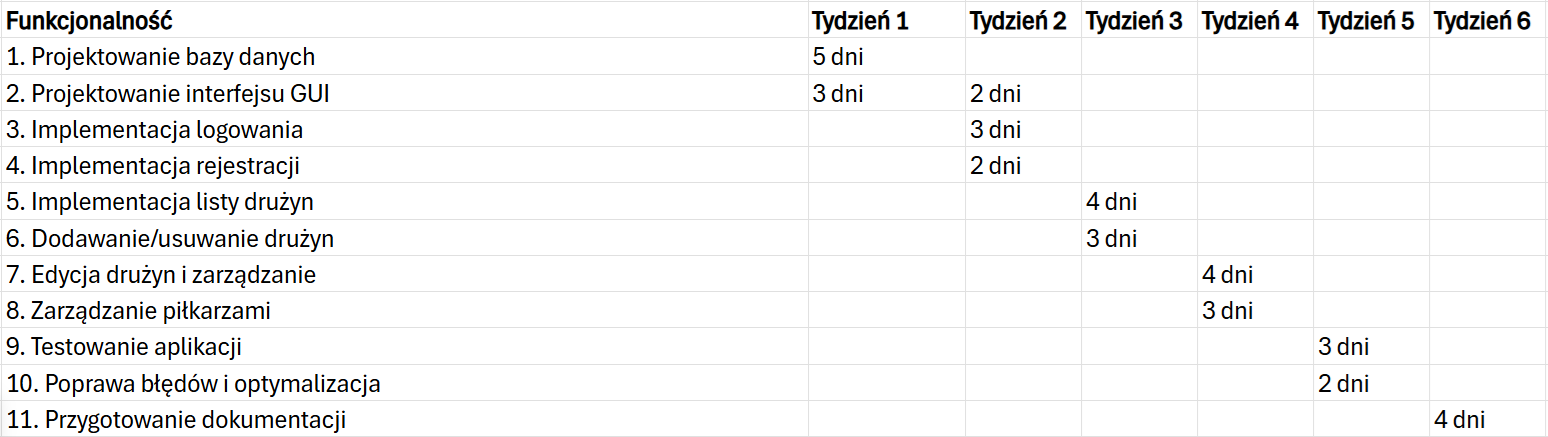
\includegraphics[width=\textwidth]{diagram.png}
    \caption{Diagram Gantta przedstawiający harmonogram realizacji projektu}
\end{figure}

Prace nad projektem rozpoczęto od zaprojektowania bazy danych oraz struktury klas aplikacji. Następnie stworzono graficzny interfejs użytkownika przy użyciu biblioteki Swing. W kolejnych etapach zaimplementowano funkcjonalności takie jak:
\begin{itemize}
    \item rejestracja i logowanie użytkownika,
    \item dodawanie, edytowanie oraz usuwanie drużyn,
    \item zarządzanie piłkarzami w drużynach,
    \item komunikacja z bazą danych oraz odświeżanie danych w GUI.
\end{itemize}

Po zakończeniu implementacji przeprowadzono testowanie wszystkich funkcji, usunięto wykryte błędy oraz przygotowano dokumentację projektu.

Do zarządzania kodem źródłowym wykorzystano system kontroli wersji \textbf{Git}. Repozytorium projektu zostało umieszczone na platformie \textbf{GitHub} pod adresem:

\begin{center}
\hypersetup{
    colorlinks=true,
    linkcolor=black,
    urlcolor=black
}
    \url{https://github.com/KubaP43/PO_Java_UR}
\end{center}

\chapter{Prezentacja warstwy użytkowej projektu}\label{4}

Aplikacja desktopowa została stworzona w języku Java z wykorzystaniem biblioteki Swing do implementacji warstwy graficznej (GUI). Umożliwia zarządzanie drużynami piłkarskimi – dodawanie, edycję oraz przypisywanie zawodników – z uwzględnieniem podziału na funkcjonalne moduły GUI.

Poniżej przedstawiono opis poszczególnych paneli aplikacji wraz z odpowiednimi zrzutami ekranu.

\begin{itemize}
  \item
  \begin{minipage}[t]{\linewidth}
    \textbf{RejestracjaGUI} -- panel służący do zakładania nowego konta. Użytkownik wprowadza nazwę użytkownika i hasło, które po zatwierdzeniu zostają zapisane w bazie danych.

    \vspace{0.3em}
    \begin{center}
      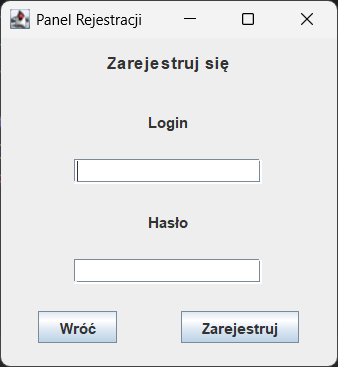
\includegraphics[width=0.7\linewidth]{rejestracja.png}
      \captionof{figure}{Panel rejestracji użytkownika (RejestracjaGUI).}
      \label{fig:rejestracja}
    \end{center}
  \end{minipage}

  \item
  \begin{minipage}[t]{\linewidth}
    \textbf{LoginGUI} -- panel logowania dla zarejestrowanych użytkowników. Po podaniu prawidłowych danych, użytkownik zostaje przekierowany do głównego interfejsu.

    \vspace{0.3em}
    \begin{center}
      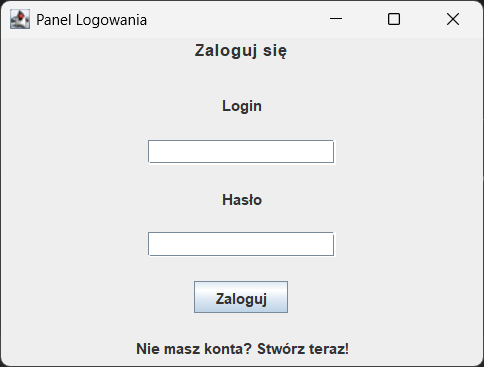
\includegraphics[width=0.7\linewidth]{logowanie.png}
      \captionof{figure}{Panel logowania użytkownika (LoginGUI).}
      \label{fig:logowanie}
    \end{center}
  \end{minipage}

  \item
  \begin{minipage}[t]{\linewidth}
    \textbf{AplikacjaGUI} -- główny panel aplikacji. Z jego poziomu użytkownik może zarządzać drużynami i zawodnikami, a także przechodzić do pozostałych funkcji systemu.

    \vspace{0.3em}
    \begin{center}
      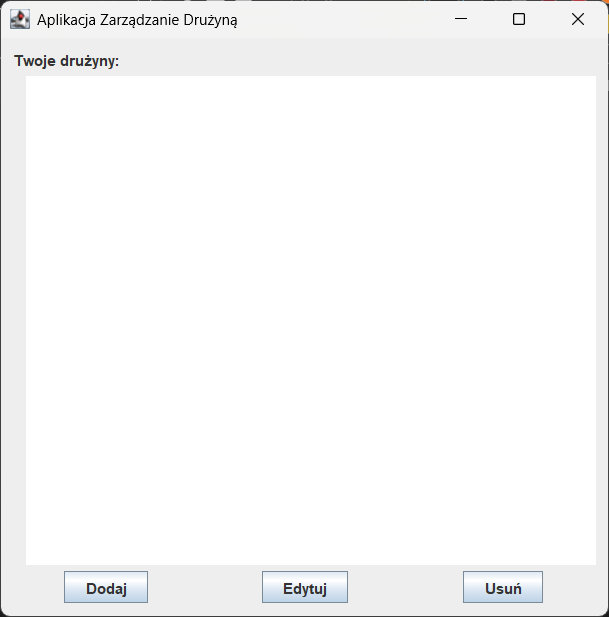
\includegraphics[width=0.7\linewidth]{panelaplikacji.png}
      \captionof{figure}{Panel główny aplikacji (AplikacjaGUI).}
      \label{fig:aplikacja}
    \end{center}
  \end{minipage}

  \item
  \begin{minipage}[t]{\linewidth}
    \textbf{DodawanieDruzynyGUI} -- panel umożliwiający dodanie nowej drużyny do systemu. Użytkownik podaje nazwę, kraj oraz inne podstawowe informacje.

    \vspace{0.3em}
    \begin{center}
      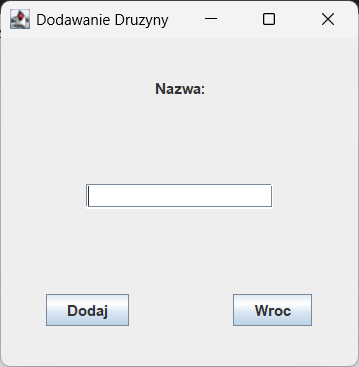
\includegraphics[width=0.7\linewidth]{dodajdruzyne.png}
      \captionof{figure}{Dodawanie nowej drużyny (DodawanieDruzynyGUI).}
      \label{fig:dodajdruzyne}
    \end{center}
  \end{minipage}

  \item
  \begin{minipage}[t]{\linewidth}
    \textbf{DodajPilkarzaGUI} -- interfejs służący do dodawania zawodników do drużyny. Można w nim określić imię, nazwisko, pozycję i inne dane piłkarza.

    \vspace{0.3em}
    \begin{center}
      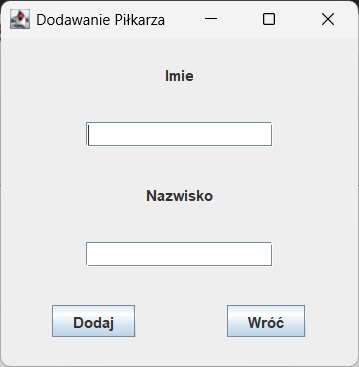
\includegraphics[width=0.7\linewidth]{dodaj pilkaza.png}
      \captionof{figure}{Dodawanie piłkarza do drużyny (DodajPilkarzaGUI).}
      \label{fig:dodajpilkarza}
    \end{center}
  \end{minipage}

  \item
  \begin{minipage}[t]{\linewidth}
    \textbf{EdytujDruzyneGUI} -- panel edycji istniejącej drużyny. Użytkownik może zmieniać dane drużyny oraz usuwać ją z systemu.

    \vspace{0.3em}
    \begin{center}
      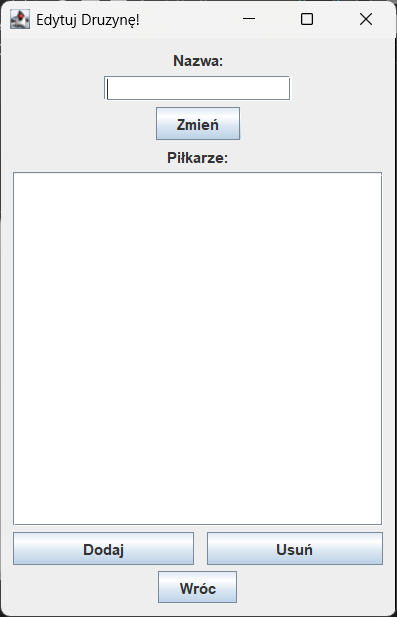
\includegraphics[width=0.7\linewidth]{edytujdruzyne.png}
      \captionof{figure}{Edycja danych drużyny (EdytujDruzyneGUI).}
      \label{fig:edytujdruzyne}
    \end{center}
  \end{minipage}
\end{itemize}

\vspace{1em}
\noindent
Cały interfejs został zaprojektowany w sposób przejrzysty i intuicyjny, z podziałem na funkcjonalne panele umożliwiające użytkownikowi pełną kontrolę nad tworzonymi danymi.

\chapter{Podsumowanie}\label{5}

W ramach projektu zrealizowano aplikację desktopową służącą do zarządzania drużynami piłkarskimi. Główne funkcjonalności obejmują możliwość rejestracji i logowania użytkownika, dodawania nowych drużyn oraz przypisywania do nich piłkarzy. Dodatkowo zaimplementowano mechanizmy edycji istniejących drużyn, a całość została zorganizowana w formie przejrzystych graficznych interfejsów użytkownika (GUI), opartych na bibliotece Swing.

Projekt został zrealizowany zgodnie z założeniami, a jego struktura umożliwia łatwą rozbudowę w przyszłości. Do najważniejszych osiągnięć należy:

\begin{itemize}
  \item zaprojektowanie i implementacja funkcjonalnych paneli GUI,
  \item integracja z bazą danych za pomocą JDBC,
  \item pełna obsługa operacji CRUD (Create, Read, Update, Delete) dla drużyn i piłkarzy,
  \item zastosowanie systemu kontroli wersji Git i współpraca zdalna za pomocą repozytorium GitHub.
\end{itemize}

Możliwe kierunki rozwoju projektu obejmują:

\begin{itemize}
  \item dodanie możliwości przeglądania szczegółowych statystyk piłkarzy i drużyn,
  \item implementację systemu logowania z poziomami dostępu (np. admin, użytkownik),
  \item rozbudowę interfejsu graficznego z wykorzystaniem nowoczesnych bibliotek JavaFX lub frameworków webowych,
  \item wdrożenie walidacji danych użytkownika i komunikatów błędów w czasie rzeczywistym,
  \item eksport danych do plików PDF lub Excel.
\end{itemize}

Zrealizowany projekt stanowi solidną podstawę pod dalszy rozwój i integrację z bardziej zaawansowanymi funkcjonalnościami w przyszłości.

\clearpage
% Dodanie spisu rysunków do spisu treści
\addcontentsline{toc}{section}{\textbf{Spis rysunków}}
\listoffigures

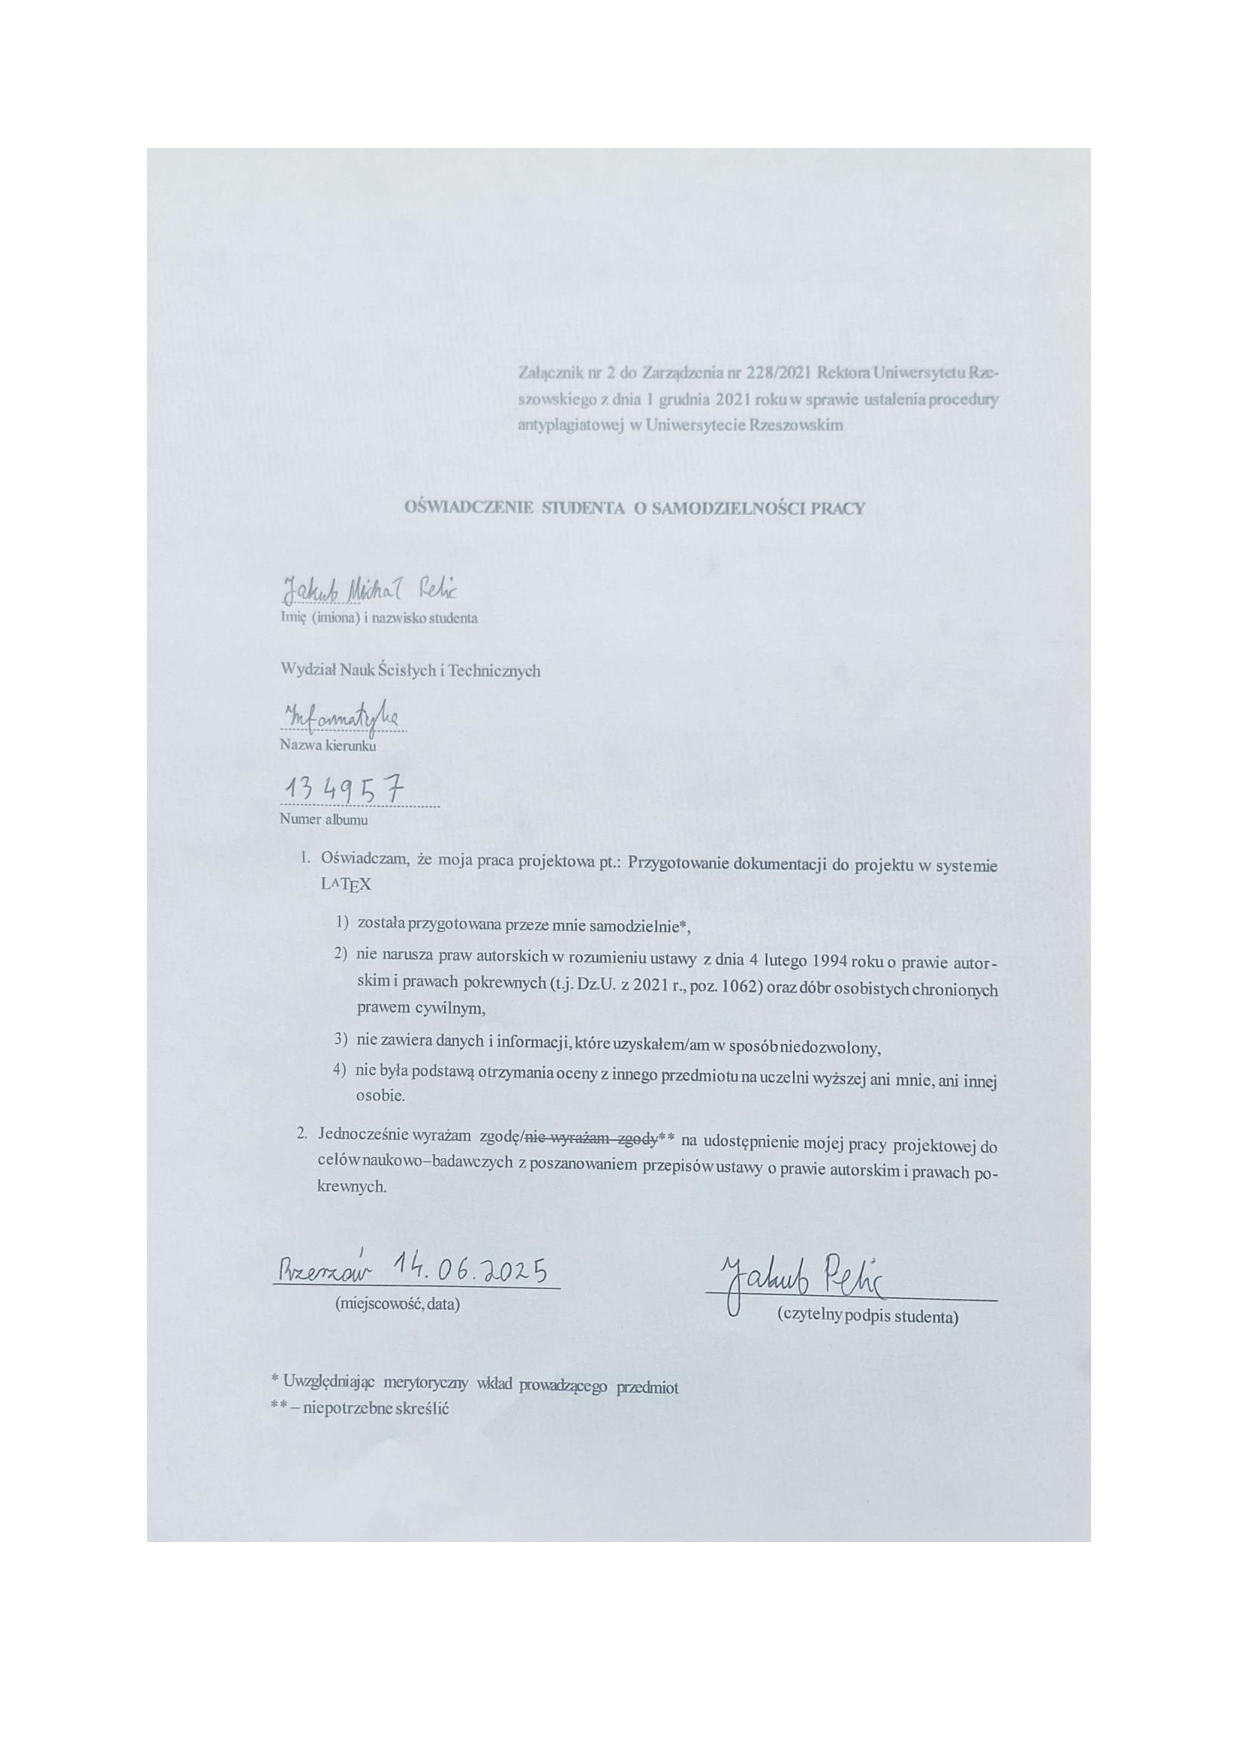
\includepdf[pages=1]{Oswiadczenie_134957.pdf}


\end{document}
